\chapter{Time Dependent Variational Principle}\label{make}
Es gibt viele Ansätze den Hamiltonian des Zentralspinmodells zu lösen, die von der exakten Lösung über 
semiklassischen Ansätzen\cite{PhysRevB.65.205309,PhysRevB.94.094308,PhysRevB.70.205327,NatalieJaeschke} bishin zum
Chebychev Expansionstheorem reichen\cite{PhysRevB.89.045317}, welche ihre eigenen Vor- und Nachteile beherbergen. 
Gerade bei einer großen Anzahl von Kernspins ist eine exakte quantenmechanische Lösung nicht anwendbar. Deshalb finden semiklassische Ansätze Verwendung, 
die eine Abweichung zur exakten Lösung in Kauf nehmen, um dafür mehr Spins behandeln zu können. \\ 
In dieser Arbeit wird das Time-Dependent Variatonal Principle, kurz TDVP, zur Lösung verwendet.
Das grundlegende Prinzip der TDVP ist die Äquivalenz der zeitabhängigen Schrödingergleichung zu einem Extremalisierungsproblem einer 
Wirkungsfunktion $S=\int_{t_1}^{t_2}L \thinspace dt$ zu nutzen. Dies kann durch die folgende Lagrange-Funktion:
\begin{align}\label{Lagrange}
    L\left(\overline{\Psi}(t), \Psi(t), t\right)=\frac{i}{2}\langle\Psi(t) \mid \dot{\Psi}(t)\rangle-\frac{i}{2}\langle\dot{\Psi}(t) \mid \Psi(t)\rangle-\langle\Psi(t)|\hat{H}(t)| \Psi(t)\rangle
\end{align}
mit einer Wellenfunktion $\ket{\Psi}$, die den ganzen Hilbertraum $H$ abdeckt, erreicht werden. \\
\noindent Um das ganze Potential des Variationsverfahren auszuschöpfen, wird sich nur auf ein Unterraum $\mathcal{M}\subset H$ des
Hilbertraumes beschränkt. Dabei kann immer noch dasselbe Verfahren für die Zeitentwicklung der Zustände $\ket{\Psi(t)}\in\mathcal{M}$
verwendet werden. Dies hat zur Folge, dass die Variation sich auf die Tangentialebene von $\mathcal{M}$ am Zustandvektor $\ket{\Psi}$
beschränkt.\\
Die Zeitabhängigkeit der Wellenfunktion $\ket{\Psi(t)}$ kann auf ein Satz von N analytischen, komplexen Parametern $\mu_i(t)$ ausgelagert werden, 
so dass $\ket{\Psi(t)} = \ket{\Psi(\mu_1(t),...,\mu_N(t))}$ gilt, wodurch auch äquivalent der Unterraum $\mathcal{M}$ definiert werden kann als:
\begin{align}
    \mathcal{M} &= \{\ket{\Psi(\vec{\mu})}|\vec{\mu}\in \mathbb{C}^N\}
\end{align}
Wird nun diese Parameterwellenfunktion, die nicht normiert sein muss, in der Lagrange-Funktion \autoref{Lagrange} verwendet, ergeben sich 
für die Parameter die \textbf{fundamentalen Bewegungsgleichungen}:
\begin{align}\label{Bewegungsgleichung}
    i\dot{\mu_i} &= \sum_{j}\left(G_{ij}\right)^{-1}\thinspace \partial_{\overline{\mu_j}}\mathcal{H}
\end{align}
mit 
\begin{align}
    G_{ij} &= \frac{\bra{\partial_{\overline{\mu_i}}\Psi}\ket{\partial_{\mu_j}\Psi}}{\N} 
    - \frac{\bra{\partial_{\overline{\mu_i}}\Psi}\ket{\Psi}\bra{\Psi}\ket{\partial_{\mu_j}\Psi}}{\N^2} \\
    \mathcal{H} &= \frac{\bra{\Psi}\hat{H}\ket{\Psi}}{\N}
\end{align}
\noindent mit der Konvention: $\bra{\partial_{\overline{\mu_j}}\Psi} = \left(\thinspace\ket{\partial_{\mu_j}\Psi}\thinspace\right)^\dagger$\\
\noindent Dabei entspricht die \textbf{modifizierte Gram-Matrix $G_{ij}$} oder Überlappmatrix der tangentialvektoren auf $\mathcal{M}$ anschaulich einer
Metrik, wenn die Tangentialvektoren linear unabhängig wären. Der \textbf{modifizierte Hamiltonian $\mathcal{H}$}, übernimmt die Rolle des eigentlichen 
Hamiltonians, wobei dieser auch die Normierung sicher stellt. \\
Eine explizite Herleitung ist in [P. Kramer and M. Saraceno, Geometry of the Time-Dependent Variational Principle in Quantum Mechanics
(Springer-Verlag, Berlin) (1981)]\cite{noauthor_2008-dn} und subsequent in Jutho Haegeman et al. „Time-Dependent Variational Principle for Quantum Lattices“\cite{Haegeman_2011} zu finden.

\newpage











\section{Wahl der Wellenfunktion für einen klassischen Ansatz}
\begin{wrapfigure}{r}{0.4\textwidth}
    \centering
    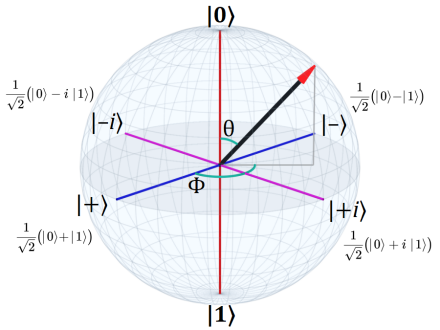
\includegraphics[width = 0.35\textwidth]{Abbildungen/bloch-sphere.png}
    \caption{Schematischer Aufbau einer Bloch-Sphere}
    \label{fig:qubit}
\end{wrapfigure}
Zur Vereinfachung werden alle Kernspins (wie der Elektronenspin) als 1/2-Spins angenähert. 
Die Wellenfunktion $\ket{\Psi}=\ket{\Psi(\mu_1(t),...,\mu_N(t)}$ enthält die zeitabhängigen Parameter $\mu_i(t)$ und realisiert einen 
kohärenten Zustand. Wir nutzen die Geometrie des 1/2-Spins aus und verwenden zur Darstellung die bekannte \textbf{Bloch-Sphäre}. 
Ähnlich wie die komplexe e-Funktion dank trigonemtrische Eigenschaften einen Kreis auf der Zahlenebene abbilden kann, ist es auch möglich,
jeden Punkt auf einer Kugel zu beschreiben. Deshalb wählen wir folgenden unnormierten Ansatz, der in den folgenden Abschnitten Verwendung 
findet:
\begin{align}\label{klassischer_Ansatz}
    \ket{\Psi(\mu_1(t),...,\mu_N(t))} &= \prod_{i=1}^{N} e^{\mu_i\thinspace S_i^-}\ket{\uparrow,...,\uparrow}
\end{align}
Dabei lässt sich diese Wellenfunktion durch diesen Normierungsfaktor normieren:
\begin{align}
    N &= \prod_{i=1}^{N} \frac{1}{\sqrt{1+\mu_i\muk_i}}
\end{align}
\section{ein 1/2-Spin im konstanten Magnetfeld}
Zum besseren Verständnis des TDVPs ist die beispielhafte Betrachtung des vereinfachten Falles sehr aufschlussreich. 
Zudem lassen sich Identitäten herleiten, die in die Erweiterung zum \textbf{Central Spin Model} Wiederverwendung finden werden. Hierfür wird nur der erste 
Summand des Zentralspinmodells betrachtet:
\begin{align*}
    \ket{\Psi} &= e^{\mu\thinspace S^-}\ket{\uparrow} \\
            &= (1 + \frac{\mu\thinspace S^{-}}{1!} + \frac{\left(\mu\thinspace S^{-}\right)^2}{2!} + ...)\ket{\uparrow}    \\
            &= \ket{\uparrow} + \mu\ket{\downarrow}
\end{align*}
\noindent Im folgenden haben wir uns die Eigenschaft des 1/2-Spins $\left(S^{-}\right)^{n}\ket{\uparrow}=0$  (n = 2,3,...) verwendet.
Der Hamiltonian lautet:
\begin{align}
    \hat{H}_1 &= \vec{b}\hat{\vec{S}} = \left(b_x\hat{S}_x+b_y\hat{S}_y+b_z\hat{S}_z \right) \\
    &= \frac{b_x}{2}\Bigl(\ket{\downarrow}\!\bra{\uparrow}+\ket{\uparrow}\!\bra{\downarrow}\Bigr) \\
    & + \frac{ib_y}{2}\Bigl(\ket{\downarrow}\!\bra{\uparrow}-\ket{\uparrow}\!\bra{\downarrow}\Bigr) \\
    & + \frac{b_z}{2}\Bigl(\ket{\uparrow}\!\bra{\uparrow}-\ket{\downarrow}\!\bra{\downarrow}\Bigr) 
\end{align}
\noindent wobei der Lande-Faktor des freien Elektrones $g_e\approx 2$ ist. 
Der Spin-Vektororperator hat die Form $\hat{\vec{S}}= \frac{1}{2}\left(\hat{\sigma}_x,\hat{\sigma}_y,\hat{\sigma}_z\right)^T$ mit den Pauli-Matrizen 
$\hat{\sigma}_i$.\\ 
und somit ergibt sich der \textbf{modifizierte Hamiltonian} und seine partielle Ableitung:
\begin{align}
    \mathcal{H} &= \frac{\gamma}{2}\frac{b_x(\mu +\muk) + ib_y(\muk - \mu) + b_z(1-\mu\muk) }{1+\mu\muk}    \\
    \partial_{\muk} \mathcal{H} &= \frac{\gamma}{2} \frac{b_x(1-\mu^2) + ib_y(1+\mu^2) - 2\mu b_z}{(1+\mu\muk)^2} 
\end{align}
\noindent Im nächsten Schritt wird die von dem Hamiltionian unabhängigen \textbf{modifizierte Gram-Matrix $G_{ii}$} bestimmt, 
welche in diesem Fall eindimesnional ist.
Damit erhalten wir
\begin{align}
    G_{11} = \frac{1}{\left(1 + \mu\overline{\mu}\right)^2} \text{\space\space bzw.\space\space } G_{11}^{-1} = \left(1 + \mu\overline{\mu}\right)^2
\end{align}
\noindent Einsetzen in die Bewegungsgleichung \autoref{Bewegungsgleichung} liefert:
\begin{align}
    i\dot{\mu_i} &= \sum_{j}\left(G_{ij}\right)^{-1}\thinspace \partial_{\overline{\mu_j}}\mathcal{H} = \left(G_{ii}\right)^{-1}\partial_{\muk} \mathcal{H} \\
    &= \frac{b_x}{2}(1-\mu^2) + \frac{i b_y }{2}(1+\mu^2) -\mu b_z   \label{Larmor} \\ 
    \leftrightarrow \dot{\mu} &= \frac{1}{2}(b_y + ib_x)\mu^2 + \frac{1}{2}(b_y - ib_x) +i\mu b_z
\end{align}
Die normierten \textbf{Spin-Erwartungswerte} $\frac{\bra{\Psi}\hat{\vec{S}}\ket{\Psi}}{\N}$ lauten:
\begin{align}
    \frac{\bra{\Psi}\hat{S_x}\ket{\Psi}}{\N} &= \frac{1}{2}\frac{\muk + \mu}{1+\mu\muk} = \frac{Re[\mu]}{1 + \mu\muk} \\
    \frac{\bra{\Psi}\hat{S_y}\ket{\Psi}}{\N} &= \frac{i}{2}\frac{\muk - \mu}{1+\mu\muk} = \frac{Im[\mu]}{1 + \mu\muk} \\
    \frac{\bra{\Psi}\hat{S_z}\ket{\Psi}}{\N} &= \frac{1}{2}\frac{1 - \mu\muk}{1 + \mu\muk}  
\end{align}
Bei dem Problem handelt es sich um die \textit{Larmor-Präzession}, indes die Lösung bereits bekannt ist. Zur Überprüfung reicht es,
 zu zeigen:
\begin{align}
    \frac{d}{dt}\left(\frac{\bra{\Psi}\hat{\vec{S}}\ket{\Psi}}{\N}\right) &= \vec{b} \cross \left(\frac{\bra{\Psi}\hat{\vec{S}}\ket{\Psi}}{\N}\right)
\end{align}
Dafür wird zuerst 
\begin{align}
    \partial_\mu \left(\frac{\bra{\Psi}\hat{S_x}\ket{\Psi}}{\N}\right)\dot{\mu} &= \frac{1}{2}\frac{1-\muk^2}{(1+\mu\muk)^2}\cdot\left[\frac{1}{2}(b_y + ib_x)\mu^2 + \frac{1}{2}(b_y - ib_x) +i\mu b_z\right] \label{dS_dmu}  
\end{align}
berechnet, um es dann in die Identität \ref{dS_dt} einzusetzen:
\begin{align}
    \frac{d}{dt}\left(\frac{\bra{\Psi}\hat{S_x}\ket{\Psi}}{\N}\right) &= \partial_{\mu}\left[\frac{\bra{\Psi}\hat{S_x}\ket{\Psi}}{\N}\right]\dot{\mu} + \partial_{\muk}\left[\frac{\bra{\Psi}\hat{S_x}\ket{\Psi}}{\N}\right]\dot{\muk}\label{dS_dt}\\
    &= b_y \frac{1}{2}\frac{1-\mu\muk}{(1+\mu\muk)^2} - b_z \frac{i}{2}\frac{\muk -\mu}{(1+\mu\muk)^2}    \\
    &= b_y\left(\frac{\bra{\Psi}\hat{S_z}\ket{\Psi}}{\N}\right) - b_z\left(\frac{\bra{\Psi}\hat{S_z}\ket{\Psi}}{\N}\right)
\end{align}
analog wird berechnet:
\begin{align}
    \frac{d}{dt}\left(\frac{\bra{\Psi}\hat{S_y}\ket{\Psi}}{\N}\right) &= b_z\left(\frac{\bra{\Psi}\hat{S_x}\ket{\Psi}}{\N}\right) - b_x\left(\frac{\bra{\Psi}\hat{S_z}\ket{\Psi}}{\N}\right)\\
    \frac{d}{dt}\left(\frac{\bra{\Psi}\hat{S_z}\ket{\Psi}}{\N}\right) &= b_x\left(\frac{\bra{\Psi}\hat{S_y}\ket{\Psi}}{\N}\right) - b_y\left(\frac{\bra{\Psi}\hat{S_x}\ket{\Psi}}{\N}\right)
\end{align}
Die Kreuzproduktstruktur lässt sich somit wiedererkennen.









%%%%%%%%%%%%%%%%%%%%%%%%%%%%%%%%%%%%












\section{Zwei Spins: Klassischer Ansatz}
Der vollständige zwei 1/2-Spin-Hilbertraum wird aufgespannt durch
\begin{align}
    \ket{\Psi} &= \alpha_1\ket{\uparrow\uparrow} + \alpha_2 \ket{\downarrow\uparrow} + \alpha_3\ket{\downarrow\uparrow} + \alpha_4\ket{\downarrow\downarrow}
\end{align}
mit den unabhängigen, komplexen Parametern $\alpha_i$.

\noindent Mit dem klassischen Ansatz $\ket{\Psi} = \ket{\Psi(\mu_1, \mu_2)}$ aus \autoref{klassischer_Ansatz} ergibt sich: 
\begin{align}
    \ket{\Psi} &= e^{\mu_1 S_{1}^{-}}e^{\mu_2 S_{2}^{-}}\ket{\uparrow,\uparrow}\\
                &= \ket{\uparrow \uparrow} +\mu_1\ket{\downarrow \uparrow} + \mu_2\ket{\uparrow \downarrow} + \mu_1\mu_2\ket{\downarrow\downarrow}\\
                &= \underbrace{\left(\ket{\uparrow}_1 + \mu_1\ket{\downarrow}_1\right)}_{\ket{\Psi_1}}\underbrace{\left(\ket{\uparrow}_2 + \mu_2\ket{\downarrow}_2\right)}_{\ket{\Psi_2}}  \\
\end{align}
Wird  die Phasenfreiheit und die Normierung berücksichtigt und unter einem komplexen Parameter $\mu_0$ zusammengefasst
\begin{align}\label{ueberlapp_klassisch}
    \underbrace{Ne^{i\phi}}_{=\mu_0}\ket{\Psi} &= \underbrace{\mu_0}_{\alpha_1}\ket{\uparrow \uparrow} 
    + \underbrace{\mu_0\mu_1}_{\alpha_2}\ket{\downarrow \uparrow} + \underbrace{\mu_0\mu_2}_{\alpha_3}\ket{\uparrow \downarrow} 
    + \underbrace{\mu_0\mu_1\mu_2}_{\alpha_4}\ket{\downarrow\downarrow}
\end{align}
lässt sich erkennen, dass die Parameter voneinander nicht unabhängig sind bzw. dass die Hyperebene für den $\alpha_1 = \mu_0 = 0$ nicht erreicht werden
kann; bis auf den trivialen Zustand null. Und genauso alle $\alpha_4$-Werte bedingt und nicht unabhängig sind. Wie sich zeigen wird, wird dadurch lediglich der klassische Unterraum 
des Hilbertraumes abgedeckt.\\
Mit diesem Produktansatz ergeben sich die \textbf{Spin-Erwartungswerte}:
\begin{align}
    \frac{\bra{\Psi}\hat{S_x}\ket{\Psi}}{\N} &= \frac{1}{2}\frac{\muk_1 + \mu_1}{1+\mu_1\muk_1} = \frac{Re[\mu_1]}{1 + \mu_1\muk_1} \\
    \frac{\bra{\Psi}\hat{S_y}\ket{\Psi}}{\N} &= \frac{i}{2}\frac{\muk_1 - \mu_1}{1+\mu_1\muk_1} = \frac{Im[\mu_1]}{1 + \mu_1\muk_1} \\
    \frac{\bra{\Psi}\hat{S_z}\ket{\Psi}}{\N} &= \frac{1}{2}\frac{1 - \mu_1\muk_1}{1 + \mu_1\muk_1}  
\end{align}
und 
\begin{align}
    \frac{\bra{\Psi}\hat{I_x}\ket{\Psi}}{\N} &= \frac{1}{2}\frac{\muk_2 + \mu_2}{1+\mu_2\muk_2} = \frac{Re[\mu_2]}{1 + \mu_2\muk_2} \\
    \frac{\bra{\Psi}\hat{I_y}\ket{\Psi}}{\N} &= \frac{i}{2}\frac{\muk_2 - \mu_2}{1+\mu_2\muk_2} = \frac{Im[\mu_2]}{1 + \mu_2\muk_2} \\
    \frac{\bra{\Psi}\hat{I_z}\ket{\Psi}}{\N} &= \frac{1}{2}\frac{1 - \mu_2\muk_2}{1 + \mu_2\muk_2}
\end{align}
Damit ergibt sich für den modifizierten Hamiltonian: 
\begin{align}
    \mathcal{H} &= \frac{\bra{\Psi}\hat{H}_1\ket{\Psi}+ \bra{\Psi}\hat{H}_2\ket{\Psi} +\bra{\Psi}\hat{H}_3\ket{\Psi}}{\N}\\
\end{align}
Mit
\begin{align}
   \bra{\Psi}\hat{H_1}\ket{\Psi} &= \frac{1}{2}(1+\mu_2\muk_2)\left(b_x(1-\mu_1^2) + ib_y(1+\mu_1^2) - 2\mu_1 b_z\right)\\
   \bra{\Psi}\hat{H_2}\ket{\Psi} &= \frac{z}{2}(1+\mu_1\muk_1)\left(b_x(1-\mu_2^2) + ib_y(1+\mu_2^2) - 2\mu_2 b_z\right)\\
   \bra{\Psi}\hat{H}_3\ket{\Psi} &= \frac{\alpha}{4}\left[( \mu_1 + \muk_1)( \mu_2 + \muk_2) - (\mu_1-\muk_1)(\mu_2 - \muk_2) + (1-\mu_1\muk_1)(1-\mu_2\muk_2)\right]
\end{align}  
Und wir erhalten die partiellen Ableitungen:
\begin{align}
    \partial_{\muk_1}\mathcal{H} &= \underbrace{\frac{1}{2(1+\mu_1\muk_1)^2}[b_x(1-\mu_1^2) + ib_y(1+\mu_1^2) - b_z\mu_1]}_{= \partial_{\muk_1} \frac{\bra{\Psi}\hat{H}_1 + \hat{H}_2\ket{\Psi}}{\N}} \nonumber\\
    &+ \underbrace{\frac{\alpha}{2}\frac{(\mu_2 -\mu_1)(1+\mu_1\muk_2)}{(1+\mu_1\muk_1)^2(1+\mu_2\muk_2)}}_{= \partial_{\muk_1} \frac{\bra{\Psi}\hat{H}_3\ket{\Psi}}{\N}}\\
    \partial_{\muk_2}\mathcal{H} &= \underbrace{\frac{z}{2(1+\mu_2\muk_2)^2}[b_x(1-\mu_2^2) + iB_y(1+\mu_2^2) - B_z\mu_2]}_{= \partial_{\muk_2} \frac{\bra{\Psi}\hat{H}_1 + \hat{H}_2\ket{\Psi}}{\N}} \nonumber \\
    &+ \underbrace{\frac{\alpha}{2}\frac{(\mu_1 -\mu_2)(1+\mu_2\muk_1)}{(1+\mu_1\muk_1)(1+\mu_2\muk_2)^2}}_{= \partial_{\muk_2} \frac{\bra{\Psi}\hat{H}_3\ket{\Psi}}{\N}}
\end{align}
Um nun die DGL aufzustellen, fehlt nur noch die Berechnung der modifizierten Gram-Matrix, die diesmal zweidimensional ist. 
Wir erhalten nach einer längeren Rechnung:
\begin{align}
    G &=
    \begin{pmatrix}
        (1+\mu_1\muk_1)^2 & 0 \\
        0 &(1+\mu_2\muk_2)^2
    \end{pmatrix} \\
    G^{-1} &=
    \begin{pmatrix}
        \frac{1}{(1+\mu_1\muk_1)^2} & 0 \\
        0 &\frac{1}{(1+\mu_2\muk_2)^2}
    \end{pmatrix}
\end{align}
\noindent Nun können die Bewegungsgleichungen aufgestellt werden:
\begin{align}
    i\dot{\mu_1} &= \sum_{j}\left(G_{1j}\right)^{-1}\thinspace \partial_{\overline{\mu_j}}\mathcal{H}  \\
    &=\underbrace{\frac{1}{2}b_x(1-\mu_1^2) + \frac{i}{2}b_y(1+\mu_1^2) -\mu_1 b_z}_{\text{Ein-Spin-Präzession um } \vec{b}} +\underbrace{\frac{\alpha}{2} \frac{(\mu_2-\mu_1)(1+\mu_1\muk_2)}{1+\mu_2\muk_2}}_{\text{Ein-Spin-Präzession um } \frac{\bra{\Psi}\hat{\vec{I}}\ket{\Psi}}{\N}  }    
\end{align}
und analoger Weise 
\begin{align}
    i\dot{\mu_2} &= \underbrace{\frac{z}{2}b_x(1-\mu_2^2) + \frac{iz}{2}b_y(1+\mu_2^2) -\mu_2 z b_z}_{\text{Ein-Spin-Präzession um } \vec{b}} +\underbrace{\frac{\alpha}{2} \frac{(\mu_1-\mu_2)(1+\mu_2\muk_1)}{1+\mu_1\muk_1}}_{\text{Ein-Spin-Präzession um } \frac{\bra{\Psi}\hat{\vec{S}}\ket{\Psi}}{\N}  }
\end{align}
\noindent Aufgrund der Linearität der Differentialgleichungen ist dank \autoref{Larmor} die Lösung der ersten beiden Summanden aus dem Ein-Spin-Fall 
zu entlesen. Nun fehlt es noch zu beweisen, dass der letztere Summand die Präzession um den Spin-Erwartungswert des jeweilig anderen Spins beschreibt. 
Wenn dieser Ansatz angenommen wird, kann dies durch Auflösen jener gezeigt werden:  
\begin{align}
     \frac{\alpha}{2}\left[\underbrace{\frac{1}{2}\frac{\mu_2 + \muk_2}{1+\mu_2\muk_2}}_{\frac{\bra{\Psi}\hat{I}_x\ket{\Psi}}{\N}}(1-\mu_1^2) 
     + i \underbrace{\frac{i}{2}\frac{\muk_2 -\mu_2}{1+\mu_2\muk_2}}_{\frac{\bra{\Psi}\hat{I}_y\ket{\Psi}}{\N}}(1+\mu_1^2) 
     - 2\mu_1\underbrace{\frac{1}{2}\frac{1-\mu_2\muk_2}{1+\mu_2\muk_2}}_{\frac{\bra{\Psi}\hat{I}_z\ket{\Psi}}{\N}} \right]
     &= \frac{\alpha}{2} \frac{(\mu_2-\mu_1)(1+\mu_1\muk_2)}{1+\mu_2\muk_2}
\end{align}
Hier lässt sich erkennen, dass die $\frac{\bra{\Psi}\hat{I_i}\ket{\Psi}}{\N}$ die Rolle des Magnetfeldes $\vec{B}$ im Ein-Spin-Lösung 
übernehmen. Wir erhalten dann aus Symmetriegründen:
\begin{align}
    \frac{d}{dt}\left[\frac{\bra{\Psi}\hat{\vec{S}}\ket{\Psi}}{\N}\right] &= \left(\vec{b} + \alpha \frac{\bra{\Psi}\hat{\vec{I}}\ket{\Psi}}{\N}\right)\cross\frac{\bra{\Psi}\hat{\vec{S}}\ket{\Psi}}{\N} \label{DGL_1}\\
    \frac{d}{dt}\left[\frac{\bra{\Psi}\hat{\vec{I}}\ket{\Psi}}{\N}\right] &= \left(z\vec{b} + \alpha \frac{\bra{\Psi}\hat{\vec{S}}\ket{\Psi}}{\N}\right)\cross\frac{\bra{\Psi}\hat{\vec{I}}\ket{\Psi}}{\N} \label{DGL_2}
\end{align}
\noindent dabei ist zu bemerken, dass $z\approx\frac{1}{800}$ klein ist, so dass im Falle des Kernspins die Heisenbergkopplung stark dominiert.\\
Wir erkennen, dass mit diesem Ansatz wie zu erwarten eine klassische Lösung erhalten, wo zwei Spins umeinander und dem Magnetfeld präzedieren. Dabei 
taucht quantenmechanische Verschränkung nicht auf, da beide Spin-Längen konstant bleiben zu jedem beliebigen Startzeitpunkt.








%%%%%%%%%%%%% Quantenkorrektur













\section{modifizierter Ansatz: Quantenkorrektur}
\noindent Wie im vorherigen Abschnitt zu sehen, erhalten wir eine klassiche Lösung. Um eine genauere Lösung zu erhalten, 
führen wir einen weiteren Korrekurparameter $\mu_{12}$ ein, wodurch ein größerer Unterraum des zwei 1/2-Spin-Hilbertraumes aufgespannt 
wird, mit der Hoffnung im Gegensatz zum klassischen Ansatz die Verschränkung zu berücksichtigen:
\begin{align}
    \ket{\Psi(\mu_1,\mu_2,\mu_{12})} &= e^{\mu_1 S_1^-}e^{\mu_2 S_2^-}e^{\mu_{12} S_1^-S_2^-}\ket{\uparrow,\uparrow}\\
                                    &= \ket{\uparrow \uparrow} +\mu_1\ket{\downarrow \uparrow} + \mu_2\ket{\uparrow \downarrow} + (\mu_1\mu_2 + \mu_{12})\ket{\downarrow \downarrow}
\end{align}
Wird  die Phasenfreiheit und die Normierung berücksichtigt und unter einem komplexen Parameter $\mu_0$ zusammengefasst
\begin{align}
    \underbrace{Ne^{i\phi}}_{=\mu_0}\ket{\Psi} &= \underbrace{\mu_0}_{\alpha_1}\ket{\uparrow \uparrow} 
    + \underbrace{\mu_0\mu_1}_{\alpha_2}\ket{\downarrow \uparrow} + \underbrace{\mu_0\mu_2}_{\alpha_3}\ket{\uparrow \downarrow} 
    + \underbrace{\mu_0(\mu_1\mu_2 + \mu_{12})}_{\alpha_4}\ket{\downarrow\downarrow}
\end{align}
wie in \autoref{ueberlapp_klassisch} lässt sich erkennen, dass die Parameter voneinander wieder nicht unabhängig sind bzw. dass die 
Hyperebene für den $\alpha_1 = \mu_0 = 0$ nicht erreicht werden kann. Dementgegend sind dafür die $\alpha_4$-Werte durch den zusätzlichen 
Parameter $\mu_{12}$ weitestgehend unabhängig, wodurch bis auf die Hyperebene alle Zustände erreicht werden sollten.    
Wir erhalten für die \textbf{Spinerwartungswerte}:
\begin{align}
    \frac{\bra{\Psi}\hat{S_x}\ket{\Psi}}{\N} &= \frac{1}{2}\frac{\muk_1 + \mu_1 + \muk_2(\mu_1\mu_2 + \mu_{12}) + \mu_2(\muk_1\muk_2 + \muk_{12})}{1+\mu_1\muk_1 + \mu_2\muk_2 + (\mu_1\mu_2 + \mu_{12})(\muk_1\muk_2 + \muk_{12})} \\
    \frac{\bra{\Psi}\hat{S_y}\ket{\Psi}}{\N} &= \frac{i}{2}\frac{\muk_1 - \mu_1 + \muk_2(\mu_1\mu_2 + \mu_{12}) + \mu_2(\muk_1\muk_2 + \muk_{12})}{1+\mu_1\muk_1 + \mu_2\muk_2 + (\mu_1\mu_2 + \mu_{12})(\muk_1\muk_2 + \muk_{12})}\\
    \frac{\bra{\Psi}\hat{S_z}\ket{\Psi}}{\N} &= \frac{1}{2}\frac{1 - \mu_1\muk_1 + \mu_2\muk_2 - (\mu_1\mu_2 + \mu_{12})(\muk_1\muk_2 + \muk_{12})}{1 + \mu_1\muk_1 + \mu_2\muk_2 + (\mu_1\mu_2 + \mu_{12})(\muk_1\muk_2 + \muk_{12})}  
\end{align}
und
\begin{align}
    \frac{\bra{\Psi}\hat{I_x}\ket{\Psi}}{\N} &= \frac{1}{2}\frac{\muk_2 + \mu_2 + \muk_1(\mu_1\mu_2 + \mu_{12}) + \mu_1(\muk_1\muk_2 + \muk_{12})}{1+\mu_1\muk_1 + \mu_2\muk_2 + (\mu_1\mu_2 + \mu_{12})(\muk_1\muk_2 + \muk_{12})} \\
    \frac{\bra{\Psi}\hat{I_y}\ket{\Psi}}{\N} &= \frac{i}{2}\frac{\muk_2 - \mu_2 + \muk_1(\mu_1\mu_2 + \mu_{12}) + \mu_1(\muk_1\muk_2 + \muk_{12})}{1+\mu_1\muk_1 + \mu_2\muk_2 + (\mu_1\mu_2 + \mu_{12})(\muk_1\muk_2 + \muk_{12})}\\
    \frac{\bra{\Psi}\hat{I_z}\ket{\Psi}}{\N} &= \frac{1}{2}\frac{1 - \mu_2\muk_2 + \mu_1\muk_1 - (\mu_1\mu_2 + \mu_{12})(\muk_1\muk_2 + \muk_{12})}{1 + \mu_1\muk_1 + \mu_2\muk_2 + (\mu_1\mu_2 + \mu_{12})(\muk_1\muk_2 + \muk_{12})}  
\end{align}
Aufgrund der Tatsache, dass bei einem freiliegenden $\vec{B}$-Feld, sich die Rechnung und Ergebnisse außerordentlich verkomplizieren ohne 
wirklich neue Physik zu bringen, wird der Einfachheit Halber das Magnetfeld in z-Richtung ausgerichtet, somit vereinfacht sich der 
Hamiltonian zu:
\begin{align}
    \hat{H} &= \vec{b}\hat{\vec{S}}_z +  z\vec{b}\hat{\vec{I}}_z + \alpha \hat{\vec{S}}\hat{\vec{I}}
\end{align}
Mit diesem Ansatz erhalten wir nach längerer Rechnung den modifizierten Hamiltonian:
\begin{align}
    \mathcal{H} &= \frac{\bra{\Psi}\hat{H}_1\ket{\Psi} +\bra{\Psi}\hat{H}_2\ket{\Psi} + \bra{\Psi}\hat{H}_3\ket{\Psi}}{\N}
\end{align}
mit 
\begin{align}
    \bra{\Psi}\hat{H}_1\ket{\Psi} &=  \frac{b}{2}\left[ 1- \mu_1\muk_1 + \mu_2\muk_2 - (\mu_1 \mu_2 + \mu_{12})(\overline{\mu_1\mu_2} + \muk_{12})\right]\\
    %
    \bra{\Psi}\hat{H}_2\ket{\Psi} &=  \frac{z b}{2}\left[ 1- \mu_2\muk_2 + \mu_1\muk_1 - (\mu_1 \mu_2 + \mu_{12})(\overline{\mu_1\mu_2} + \muk_{12})\right] \\
    %
    \bra{\Psi}\hat{H}_3\ket{\Psi} &= \frac{\alpha}{4}[2(\muk_1\mu_2 + \mu_1\muk_2) + 1 - \mu_1\muk_1 - \mu_2\muk_2 + (\mu_1 \mu_2 + \mu_{12})(\overline{\mu_1\mu_2} + \muk_{12})]
\end{align}
\noindent Damit folgen für die partiellen Ableitungen nach den konjugierten Parameter
\begin{align}
    \partial_{\muk_1} \mathcal{H} &= 
    -b \frac{\mu_1(1+\mu_2\muk_2)^2 + \muk_2\mu_{12}}{\N^2}\nonumber\\
    &+z b \frac{\muk_{12}(\mu_1\mu_2 + \mu_{12})}{\N^2}\nonumber\\
    &+\frac{\alpha}{2}\frac{(\mu_2-\mu_1)(\mu_1\muk_2+1)(1+\mu_2\muk_2)+\muk_{12}(\mu_1\mu_2 + \mu_{12}) + \mu_{12}\muk_2}{\N^2}\label{dH_Q1} \\
    %
    \partial_{\muk_2} \mathcal{H} &= 
    +b \frac{\muk_{12}(\mu_1\mu_2 + \mu_{12})}{\N^2} \nonumber\\
    &-z b \frac{\mu_2(1+\mu_1\muk_1)^2 + \muk_1\mu_{12}}{\N^2} \nonumber\\
    &+\frac{\alpha}{2}\frac{(\mu_1-\mu_2)(\mu_2\muk_1+1)(1+\mu_1\muk_1)+\muk_{12}(\mu_1\mu_2 + \mu_{12}) + \mu_{12}\muk_1}{\N^2} \\
    %
    \partial_{\muk_{12}} \mathcal{H} &= 
    -b\frac{(\mu_1\mu_2+\mu_{12})(1+\mu_2\muk_2)}{\N^2} \nonumber\\
    &-zb\frac{(\mu_1\mu_2+\mu_{12})(1+\mu_1\muk_1)}{\N^2} \nonumber\\
    &+\frac{\alpha}{2}\frac{(\muk_1-\muk_2)(\mu_1-\mu_2)(\mu_1\mu_2+\mu_{12})}{\N^2}\label{dH_Q12}
\end{align}
\noindent Und für die Gram-Matrix erhalten wir:
\begin{align}\label{Gram_Korrektur}
    G &=
    \begin{pmatrix}
        (1+\mu_1\muk_1)^2 + \mu_{12}\muk_{12} & -\mu_1^2\muk_{12} - \muk_2^2\mu_{12} &  \mu_2(1+\mu_2\muk_2)-\muk_1\mu_{12}\\
        -\mu_2^2\muk_{12} - \muk_1^2\mu_{12} &(1+\mu_2\muk_2)^2 + \mu_{12}\muk_{12} & \mu_1(1+\mu_1\muk_1)-\muk_2\mu_{12}\\
        \muk_2(1+\mu_2\muk_2)-\mu_1\muk_{12} & \muk_1(1+\mu_1\muk_1)-\mu_2\muk_{12} & 1 + \mu_1\muk_1 + \mu_2\muk_2
    \end{pmatrix}\frac{1}{\N^2} 
\end{align}
Somit lassen sich die Bewegungsgleichungen der Parameter explizit aufschreiben:
\begin{align}
    i\dot{\mu}_1 &= G_{1,1}^{-1}\thinspace \partial_{\muk_1}\mathcal{H} + G_{1,2}^{-1}\thinspace\partial_{\muk_2}\mathcal{H} + G_{1,3}^{-1}\thinspace\partial_{\muk_3}\mathcal{H}\label{QK_DGL1} \\
    i\dot{\mu}_2 &= G_{2,1}^{-1}\thinspace\partial_{\muk_1}\mathcal{H} + G_{3,2}^{-1\thinspace}\partial_{\muk_2}\mathcal{H} + G_{2,3}^{-1}\thinspace\partial_{\muk_3}\mathcal{H} \\
    i\dot{\mu}_{12} &= G_{3,1}^{-1}\thinspace\partial_{\muk_1}\mathcal{H} + G_{3,2}^{-1}\thinspace\partial_{\muk_2}\mathcal{H} + G_{3,3}^{-1}\thinspace\partial_{\muk_3}\mathcal{H} \label{QK_DGL3}
\end{align}




